\documentclass{article}
\usepackage[T1]{fontenc}
\usepackage{microtype,graphicx,booktabs,amsmath}
\usepackage[hypertexnames=false]{hyperref}
\usepackage[accepted]{mlsys2025}
\hypersetup{pdftitle={A Study of Prefix Sharing in LLM Serving},pdfsubject={Rice University COMP536 final project},pdfauthor={Thomas Lin; Yu-Ting Chung; Patrick Chiou; Yu-Xin Lai}}
\mlsystitlerunning{A Study of Prefix Sharing in LLM Serving}
\makeatletter
\renewcommand{\Notice@String}{Rice University, COMP536 course project, November 2026.}
\renewcommand{\printAffiliationsAndNotice}[1]{\begingroup\renewcommand{\thefootnote}{}\footnotetext{\textsuperscript{1}Rice University. \Notice@String}\endgroup}
\makeatother
\begin{document}
\twocolumn[
\mlsystitle{A Study of Prefix Sharing in LLM Serving}
\begin{mlsysauthorlist}
\mlsysauthor{Thomas Lin}{rice}
\mlsysauthor{Yu-Ting Chung}{rice}
\mlsysauthor{Patrick Chiou}{rice}
\mlsysauthor{Yu-Xin Lai}{rice}
\end{mlsysauthorlist}
\mlsysaffiliation{rice}{Rice University}
\begin{center}\small \texttt{tl183@rice.edu, yc223@rice.edu, pc82@rice.edu, yl371@rice.edu}\end{center}
\vskip .08in
\begin{abstract}
Prefix caching avoids repeated prefill work, but its effectiveness depends on capacity, block granularity and workload locality. We implement a CPU trace executor within vLLM v0's online serving path, retaining scheduling, sequence management and virtual prefix-block allocation. We evaluate matched single- and multi-turn ShareGPT workloads over 108 configurations, reuse a validated eight-source, 51-configuration baseline study, and evaluate eight policies on two mixed-workload compositions. With LRU/block 16, matched single/multi means are 4.41\%/3.52\% at 0.05\,GiB. Coding-agent LRU exceeds LFU by 13.16\,pp. Highest observed mixed scores are RFIFO 60.25\% (skewed) and RFIFO 41.18\% (equal-token). The simulator passes 146 correctness tests including both API frontends after repairing workload-label transport through multiprocessing. Results characterize realized cache reuse under controlled trace replay rather than GPU latency or throughput; limited production windows and single-seed mixed comparisons constrain generalization.
\end{abstract}
\vskip .12in]
\printAffiliationsAndNotice{}

\section{Introduction}
LLM serving repeatedly processes instructions, documents and conversation histories that share input prefixes. Prefill constructs attention key/value (KV) state; subsequent decoding extends it. Retaining identical full-prefix KV blocks lets later requests avoid redundant prefill. PagedAttention provides block-based memory management and sharing in vLLM \citep{kwon2023}. Which reusable blocks remain available depends on both workload arrival structure and eviction decisions under limited capacity.

Different workloads create different retention problems. Growing conversations often revisit recently extended histories; a common instruction may recur across many otherwise unrelated requests; document questions can concentrate reuse in short bursts. This motivates three questions: can CPU trace replay preserve the online serving control flow, how do capacity and block size affect realized sharing in homogeneous chat, and which eviction rules work across heterogeneous and mixed workloads?

We contribute an online trace executor, causal client and request/block metrics, then compare homogeneous chat, eight separate sources and eight policies under two mixtures. Policy orderings are configuration-specific.

\section{Background and Related Work}
A KV block depends on its preceding token prefix: identical chunks in different histories are not generally interchangeable. Reference-counted active blocks are not candidates for eviction; policies order unused cached content. LRU favors recent access, LFU allocator access frequency, and FIFO insertion order. Their usefulness depends on whether past recency, popularity or insertion age predicts future demand.

vLLM's PagedAttention addresses block allocation and sharing \citep{kwon2023}. SGLang uses RadixAttention for reuse across structured programs \citep{sglang}; Prompt Cache uses explicitly defined reusable modules \citep{promptcache}. CacheBlend addresses non-prefix retrieval chunks with selective recomputation \citep{cacheblend}, whereas our simulator retains exact full-prefix semantics. Mooncake studies KV-centric disaggregated serving \citep{mooncakepaper}; our use of released anonymous hashes does not reproduce its distributed architecture. We study replacement behavior inside an existing serving control path, not a new attention algorithm or GPU serving speedup.

\section{System Design and Implementation}
\subsection{Trace execution within online serving}
The ordinary path accepts OpenAI-compatible HTTP requests, preprocesses prompts, admits sequence groups, schedules iteration-level work, manages KV blocks, executes a model and processes token outputs. Our \texttt{SimExecutor}/\texttt{SimExecutorAsync} replaces model execution with \texttt{Simulator.step}; the surrounding v0 components remain active. Workload metadata and executor selection are modified, so the scheduler is not claimed entirely unchanged. Figure~\ref{fig:architecture} contrasts the execution backends and illustrates exact prefix sharing.

\begin{figure*}[t]
\centering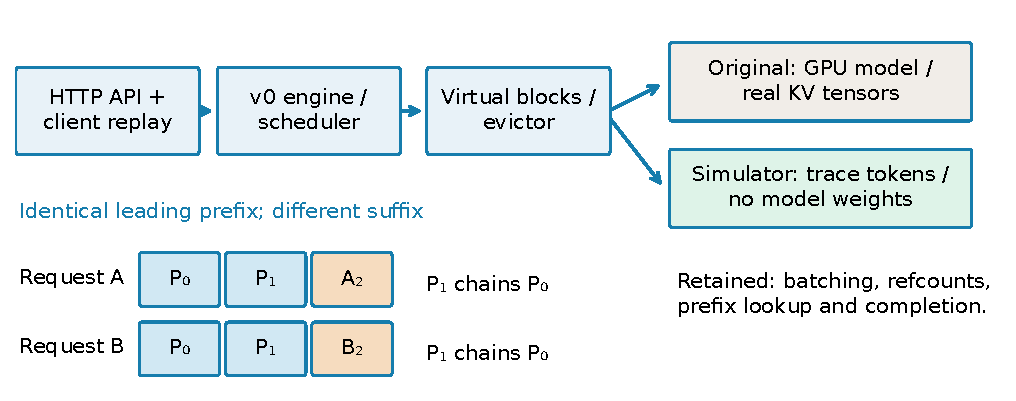
\includegraphics[width=.95\textwidth]{figures/system_prefix.pdf}
\caption{Retained online control path with GPU execution replaced by trace replay. Identical leading token blocks share KV state; a changed suffix is computed separately. Chained identity prevents sharing an identical local block after a different prefix.}
\label{fig:architecture}
\end{figure*}

The simulator consumes full scheduled metadata, honors \texttt{do\_sample}, accounts for computed blocks during prefill and returns compatible sampler outputs. Next-token selection uses the existing output length, avoiding response restart after recomputation. Fully cached prompts still recompute the final token for sampling. Standard output processing enforces EOS/stop handling and releases completed/aborted request state. Strict trace lookup matches prompt tokens and request IDs; duplicate prompts with different recorded replies therefore remain distinguishable.

No model weights, attention kernels or actual KV tensors are loaded. Configuration and tokenizer files remain necessary. Virtual KV bytes per block are
\begin{equation}
B_{\rm KV}=2 L H_{\rm KV}d_h b s,
\end{equation}
where $L$ is attention layers, $H_{\rm KV}$ KV heads per rank, $d_h$ head dimension, $b$ tokens/block and $s$ bytes/element. This geometry controls virtual capacity, not allocated GPU memory. The executor awaits synthetic costs of 0.01\,ms per uncached prefill token and 0.1\,ms per decode sequence-step. CPU/HTTP overhead and queuing remain real wall time. LoRA, prompt adapters, speculative decoding and multistep scheduling are unsupported in this executor.

\subsection{Client, traces and workload labels}
\texttt{TraceBuilder} reuses serving preprocessing and the model's chat template/tokenizer, with fixed date arguments. ShareGPT normalization enforces role ordering and filters whole conversations for context eligibility. Single-turn mode retains only the first user/reply pair; multi-turn retains all eligible turns. The two modes thus share the same initial conversations and first-turn prompts/target arrivals. Optional agent truncation retains a causal prefix.

The client uses recorded times or seeded exponential interarrivals for a Poisson process. It limits concurrency and waits for each preceding reply before a later turn, preserving causality even if desired arrivals are already past. It checks response text, token counts and finish reason; failed turns prevent descendants. Dispatch lag distinguishes target arrival rate from achieved sends.

Dataset-provided labels propagate through request, sequence and block metadata; no online workload classifier is implemented. A missing optional label remains \texttt{None}. We repaired an incomplete multiprocessing path by adding the label to the client method, pickled RPC request and engine-side submission, rather than dropping it or disabling the frontend. Both endpoints/frontends now pass integrated request/block-label checks. Full simulator correctness evidence is 146 passing tests, including trace identity, batching, EOS, preemption/recomputation and eviction ordering. This validation is scoped to the simulator suite, not all GPU-dependent upstream tests.

\subsection{Custom eviction policies}
TLRU orders three tiers: one-shot/expired/over-budget blocks first, recent agent/Bailian blocks next, and cross-label shared blocks last; recency orders each tier. Its hold is 8 seconds and protected budget 1 of the current unused-block table. TFIFO uses the same label tiers with insertion order and no expiry. Both classify chat as one-shot in the implemented static rule.

HFIFO and HLRU are label independent: a block's first reuse promotes it, with FIFO ordering or recency plus hold/budget expiry. RFIFO tracks100 resolved block outcomes per label (first hit, or eviction without a hit). Once full, a window with at least 5\% hits admits new blocks to a protected FIFO tier if any label qualifies. Later hits do not promote already resident low-tier blocks. These rules prioritize victims rather than absolutely pinning protected content: if lower tiers are empty, a protected unused block is evicted. Heap/version bookkeeping usually costs logarithmic operations, with stale-pop/rebuild worst cases; RFIFO also stores100 outcomes per label. Detailed state and pseudocode appear in the appendix.

\section{Experimental Methodology}
\subsection{Workloads and controlled configurations}
All studies use Qwen/Qwen2.5-0.5B-Instruct and tokenizer revision \texttt{7ae5576\ldots}, CPU-only v0 online simulation. M2 recovers the documented absolute-capacity sweep:200 eligible ShareGPT conversations, context 4096, single/multi modes,0.05/0.10\,GiB,8/16/32 tokens per block, LRU/LFU/FIFO, target100 requests/s, concurrency/max-sequences64, think time 0 and seeds 0/1/2. This gives108 configurations. Byte capacity is held approximately constant across block sizes (whole-block rounding); no ratio-based fallback is mixed into these comparisons. M2-A reuses block 16 LRU cells from M2-B.

The separate-source Task 1 study uses 51 existing configurations with 16-token blocks, cache approximately 25\% of each source's distinct full-block working set and concurrency 8. Text sources are ShareGPT \citep{sharegpt}, four interleaved AgentBank tasks \citep{agentbank}, CC-Bench coding trajectories \citep{ccbench}, grouped QuALITY document questions \citep{quality} and Code Alpaca instructions \citep{codealpaca}. Bailian chat/coder and Mooncake tool-agent windows provide anonymized prefix hashes \citep{bailian,mooncake}. Contexts are 2048 for chat/AgentBank,8192 for coding/QuALITY,32768 for production hashes and 1024 for code. Text uses 2--3 arrival seeds; production windows use one.

Hash traces map to deterministic synthetic token blocks; output filler is capped at 32 tokens. Bailian times are scaled by 0.25 and Mooncake by 0.5; Mooncake has512-token hashes and millisecond timestamps. Agent conversion omits original system/tool schemas; CC conversion excludes thinking/images/sub-agent branches and truncates long contexts. QuALITY interleaves groups of ten articles. These transformations define the studied workload rather than an exact production replica.

Mixed trials use one common context 32768, block 16, cache ratio 0.10, target100 requests/s, concurrency 8 and think time 1 second. The skewed cohort reuses the original construction; the equal-token cohort takes each label's first causal prefix reaching260,000 prompt tokens, with final-turn overshoot recorded. Mixed preparation retags IDs, shuffles conversations and assigns new Poisson first-turn times, discarding recorded production times. All policies see identical prepared hashes/capacity in each mixture. Each starts a fresh server/cache; new policy order is randomized. We complete one seed per mixture for all eight policies before any optional repetition, totaling 16 runs. The two-core/8\,GiB environment and recorded run times favor complete required comparisons over large ablation products; no mixed confidence interval is inferred.

\begin{table}[t]
\centering\small
\caption{Primary controls. M2 uses blocks8/16/32; others16. Seeds vary arrival timing, not dataset sampling.}
\begin{tabular}{lrrrl}\toprule
Study & Context & Cache & Conc. & Seeds\\\midrule
M2 & 4096 & .05/.10 GiB & 64 & 3\\
Task 1 & 1024--32768 & .25 ratio & 8 & 1--3\\
Mixed & 32768 & .10 ratio & 8 & 1\\\bottomrule
\end{tabular}
\end{table}

\subsection{Metrics, integrity and reproducibility}
For request $i$, sharing fraction is $f_i=C_i/P_i$, where $C_i$ and $P_i$ are cached and total prompt tokens. The primary aggregate is
\begin{equation}
S=\frac{\sum_i C_i}{\sum_i P_i},
\end{equation}
which differs from the mean-request fraction $N^{-1}\sum_i f_i$. We report percentage-point (pp) changes separately from relative changes against a nonzero, configuration-matched baseline. Repeated-seed means use sample SD; one-run mixed/production results have no variability estimate or significance claim.

A logical full block is identified by a SHA256 chain over the preceding prefix and current tokens. Hits count distinct requests skipping that block at initial prefill and include zero-hit blocks in the population. Decode-computed blocks are also observed; counts aggregate across cache residencies. Reuse gaps are monotonic wall time since the preceding distinct-request access \emph{sampled at successful hits}; they exclude missed reuse and are not unconditional recurrence distributions or GPU times.

Per-run manifests record commands, source/input fingerprints, versions, seeds, capacity and controls alongside raw request/block logs. Independent analysis checks complete cohorts, IDs, token arithmetic, hit/gap totals, causality and policy input/capacity equality. Interrupted attempts are retained and excluded. All175 studied configurations pass exported consistency checks; raw request totals include repeated replays of the same cohorts, not independent dataset samples. New mixed trials additionally count successful eviction allocations with an opt-in wrapper that preserves allocator results/ordering; its isolated check passes. Historical M2/Task 1 eviction counts and all promotion counts are unavailable rather than inferred from misses.

\section{Experimental Results}
\subsection{Homogeneous conversation reuse}
At block 16 with LRU, single-turn sharing is (4.41 $\pm$ 0.01)\% at 0.05\,GiB versus multi-turn (3.52 $\pm$ 0.00)\%. At0.10\,GiB, the corresponding means are (4.41 $\pm$ 0.01)\% and (4.71 $\pm$ 0.16)\% (Figure~\ref{fig:m2mode}). Each mode starts from 200 identical eligible conversations; single runs contain200 requests and multi runs608. All three arrival seeds use the same tokenized cohorts. These are observations under the documented64-concurrent-request load, not an assumption that multi-turn must improve sharing. Representative seed 0 request-fraction medians are 24.07\% single and 2.58\% multi; the logical-block hit median is zero in both. These populations differ from token weighting. At block 16 the two capacities hold273/546 virtual blocks (4,368/8,736 tokens), small relative to 64 active sequence slots. A policy-independent diagnostic finds 4.65\% single-turn and 57.73\% multi-turn prompt tokens in full blocks seen in an earlier planned prompt. It omits decode blocks, availability and actual completion timing, so it is not a full-serving cache bound. The large multi-turn recurrence versus low realized sharing distinguishes existing overlap from retained state.

\begin{figure*}[t]
\centering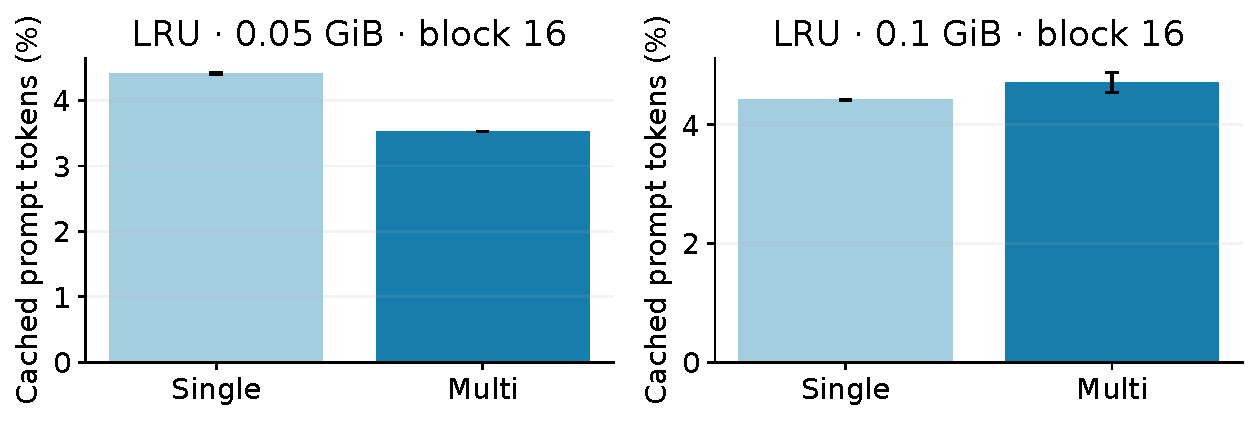
\includegraphics[width=.73\textwidth]{figures/m2_single_multi.pdf}
\caption{Matched single/multi ShareGPT cohorts, LRU/block 16. Bars are mean token-weighted sharing and whiskers sample SD over three arrival seeds; capacities are absolute virtual GiB. More conversational history does not imply a larger realized token-weighted fraction under the tested cache and load.}
\label{fig:m2mode}
\end{figure*}

Per-request CDFs, block-hit counts and hit-associated gap distributions provide complementary populations (appendix). Long prompts receive greater weight than in a median-request statistic. Only complete prefixes surviving allocation pressure become hits. Arrival, concurrency and causal completion affect survival; this interpretation is not an isolated causal ablation.

\subsection{Capacity and block granularity}
At0.05\,GiB, LRU scores at 8/16/32 tokens per block are 6.61\%, 4.41\%, 0.01\% for single-turn and 4.83\%, 3.52\%, 1.50\% for multi-turn. Doubling byte capacity changes block 16 LRU by +0.00\,pp (single) and +1.18\,pp (multi). Figure~\ref{fig:sensitivity} shows the other policies and seed variability; the complete36-cell mean/SD table is supplementary. In single-turn/block 8 at 0.05\,GiB, FIFO reaches (6.61 $\pm$ 0.01)\%, versus LRU (6.61 $\pm$ 0.01)\% and LFU (6.61 $\pm$ 0.01)\%. The observed ranking therefore interacts with granularity; the study does not isolate a causal retention mechanism.

\begin{figure*}[t]
\centering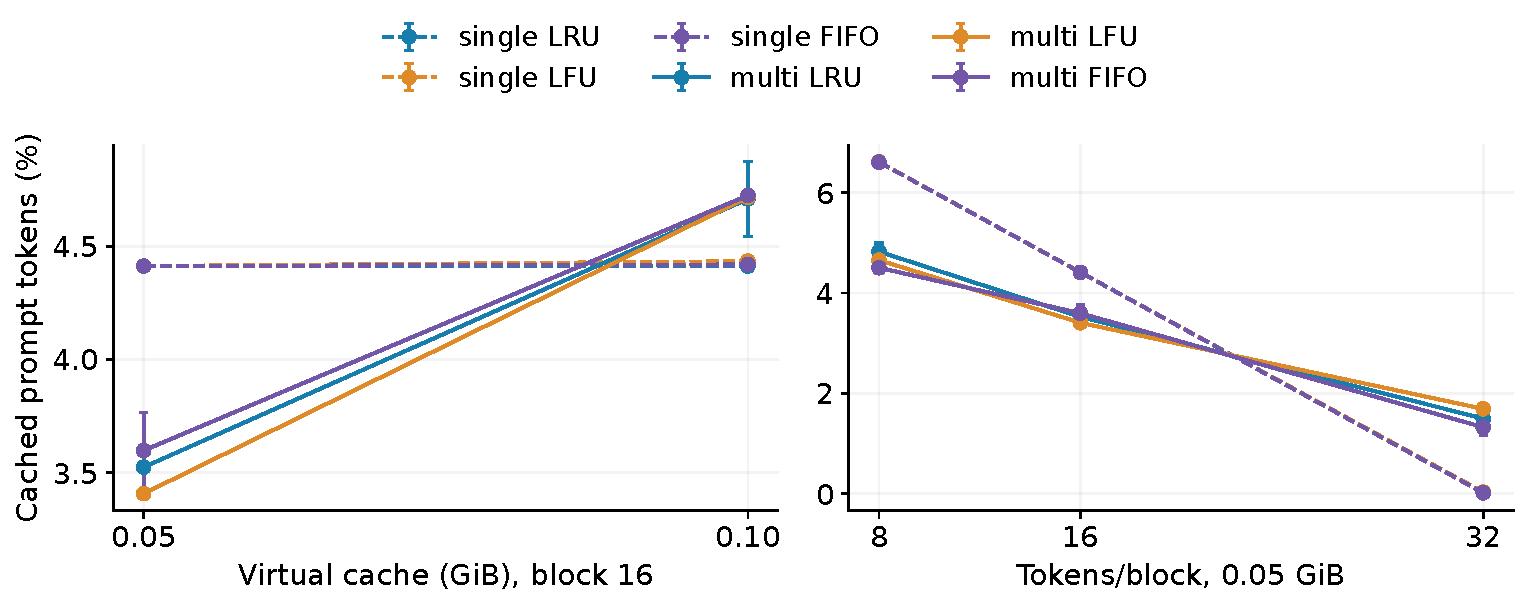
\includegraphics[width=.95\textwidth]{figures/m2_sensitivity.pdf}
\caption{M2 sensitivity under approximately fixed bytes across block sizes. Capacity panel holds block 16; granularity panel holds0.05\,GiB. Solid lines: multi; dashed: single. Colors identify policies; points/whiskers are seed means/sample SD. Only two capacities are tested, so a general saturation curve is not established.}
\label{fig:sensitivity}
\end{figure*}

A larger block matches a coarser full-prefix unit and leaves longer non-full tails that cannot be reused. Code/role/template prefixes shorter than32 tokens may therefore contribute at 8/16 but not32. This explains a possible mechanism for the measured granularity effect; it does not by itself quantify allocator overhead or GPU efficiency. Larger capacity can preserve more useful prefixes, but changing scheduling/preemption and realized order can prevent simple monotonicity. We report the observed cells rather than imposing a trend.

\subsection{Separate heterogeneous workloads}
Figure~\ref{fig:task1} uses the validated51-run study (21,834 successful requests, zero failures); the multiprocessing-only transport fix does not alter its direct-mode executor/cache decisions. Coding-agent LRU reaches48.59\% versus 35.43\% for LFU and 47.35\% for FIFO, approximately 13.16\,pp above LFU. Growing contexts plausibly favor retention of recently added prefixes while frequency can favor older popular blocks; no mechanism ablation proves this explanation.

LFU leads the observed Bailian chat/coder windows (29.52\%/37.28\%) versus LRU 28.44\%/35.87\% and FIFO 26.75\%/32.88\%. Each has one run, so production-wide superiority is not established. QuALITY FIFO 50.35\% exceeds LRU 49.25\% and LFU 45.54\%, with small repeat counts. AgentBank LRU 50.55\% and LFU 50.47\% differ by only 0.074\,pp. Mooncake LRU 40.27\% and LFU 40.25\% nearly tie; FIFO 39.72\%. ShareGPT is seed-sensitive; Code Alpaca ties at 29.53\% for all policies. Cross-workload capacities/contexts differ, so these establish within-source choices rather than a causal workload ranking.

\begin{figure*}[t]
\centering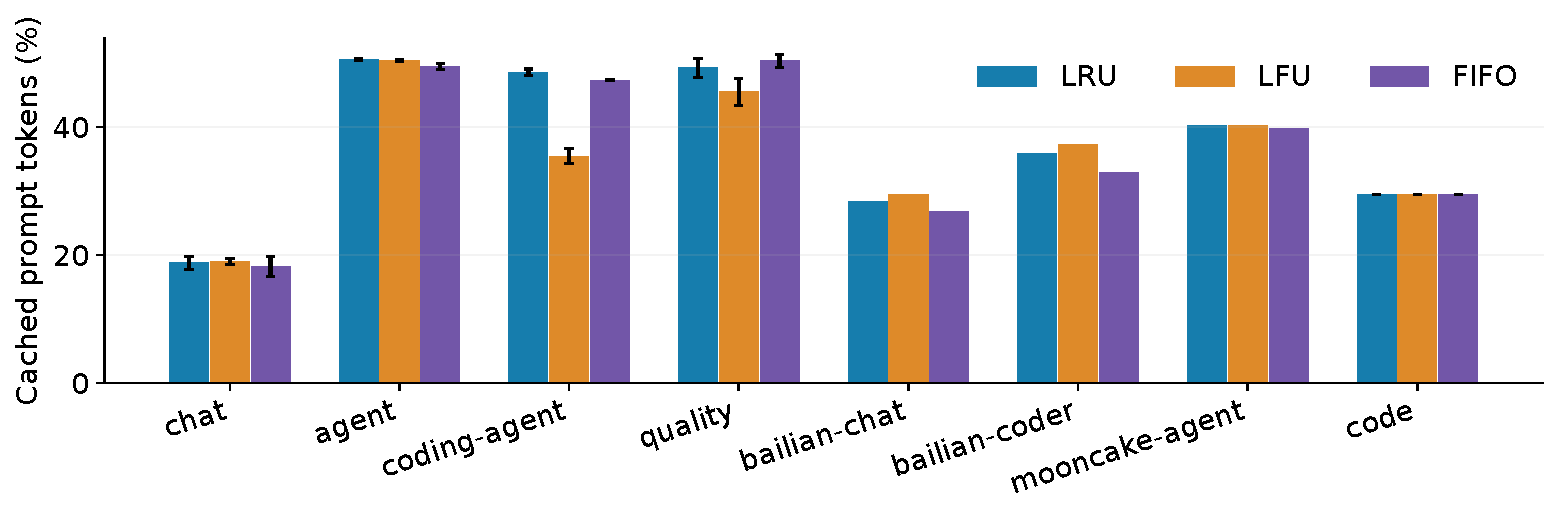
\includegraphics[width=.95\textwidth]{figures/m3_task1.pdf}
\caption{Separate-workload baseline sharing, cache ratio 0.25/block 16. Whiskers are sample SD for 2--3 arrival seeds; production windows have $n=1$ and unknown variability. Highest observed policy and best--second gaps are tabulated in the appendix.}
\label{fig:task1}
\end{figure*}

Representative LRU seed 0 distributions show concentrated reuse: zero-hit logical blocks are 87.23\% chat,76.56\% AgentBank,58.02\% coding-agent and 20.37\% QuALITY. Median hit-associated gaps are 0.210,0.017,1.012 and 0.177 seconds respectively. These retained-prefix observations motivate recency/frequency/admission comparisons, but cannot directly set a universal hold duration because gaps are survival-conditioned and wall-clock dependent.

\subsection{Mixed-workload policies}
The skewed mixture contains 3,322 requests and 10,517,812 prompt tokens, with 12,360 virtual blocks. Its highest observed policy is RFIFO at 60.25\%, compared with strongest baseline FIFO at 49.12\%: +11.13\,pp, or 22.66\% relative using unrounded scores. This single-run margin has no SD/CI estimate.

The equal-token mixture contains 6,051 requests and 2,119,769 prompt tokens, with 8,043 virtual blocks. Its highest observed policy is RFIFO at 41.18\%, compared with strongest baseline LRU at 35.85\%: +5.33\,pp, or 14.87\% relative using unrounded scores. This single-run margin has no SD/CI estimate.

\begin{figure*}[t]
\centering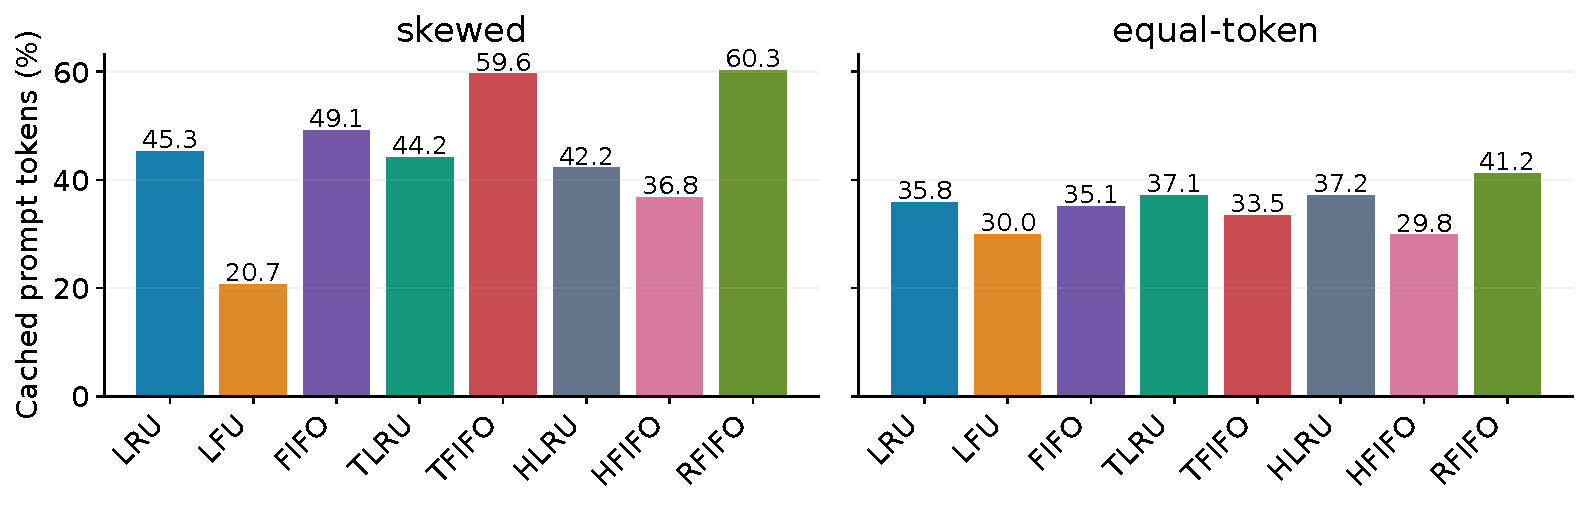
\includegraphics[width=.90\textwidth]{figures/mixed_overall.pdf}
\caption{Newly validated mixed-workload scores for eight policies, common within-mixture inputs/capacity and randomized execution order. One seed per mixture; no error bars or statistical-superiority claim. Full per-label scores and request/token composition are in the appendix.}
\label{fig:mixed}
\end{figure*}

TFIFO changes from 59.58\% on the skewed mix to 33.46\% on equal tokens; RFIFO changes from 60.25\% to 41.18\%. The per-label chat comparison is skewed: TFIFO chat2.44\% versus baseline2.71\%; equal-token: TFIFO chat4.02\% versus baseline48.33\%. Static treatment of chat as one-shot can therefore be evaluated against measured category effects rather than inferred from the aggregate alone. Dataset composition, hold expiration and adaptive admission offer plausible mechanisms; there is no held-out tuning/ablation study establishing causation. The new raw-validated scores replace documentary historical values rather than being adjusted to reproduce them. On skewed, the aggregate winner's largest category decline versus the strongest baseline is bailian-coder, -14.72\,pp; aggregate improvement does not protect every category. On equal-token, the aggregate winner's largest category decline versus the strongest baseline is mooncake-agent, -4.83\,pp; aggregate improvement does not protect every category.

\section{Discussion and Limitations}
The experiments establish workload/configuration-dependent realized reuse, not one optimal eviction rule. Static labels can preserve useful agent prefixes in one composition while harming a returning conversational category in another; adaptive admission can alter that trade-off without a universal guarantee. Labels are known from data, not predicted. Hold expiration depends on real CPU queuing and HTTP/synthetic delay. Single-seed mixed comparisons, fixed time windows, first-eligible subsets, one mixed pressure level and absent ablations limit external validity. Changing mixture also changes selected cohorts and absolute bytes at the fixed ratio, so this is not a composition-only causal ablation. Optional parameter tuning was not prioritized over required complete comparisons.

The simulator does not model logits, numerical model quality, GPU bandwidth/kernels, real device timing or distributed KV transfer. Reuse scores cannot be converted directly into GPU speedups. CDFs of realized hits exclude missed opportunities; transformed traces omit original agent prompts and shorten production outputs. All trace entries are loaded into memory.

\section{AI Assistance}
Codex assisted code generation and bug fixes (including multiprocessing labels), tests, experiment scripts, validation, data organization, figures, report and presentation preparation. Automated checks do not establish human review; historical AI use outside this conversation is unconfirmed. Significant user prompts appear in the appendix.

\section{Conclusion}
The CPU executor preserves an active online scheduling/cache path while substituting trace tokens for model computation. Matched chat reuse changes with block/byte controls, while heterogeneous policies range from large coding-agent differences to near ties. Highest observed mixed policies are RFIFO on skewed and RFIFO on equal-token input, with single-seed uncertainty. The findings support conditional policy selection and further controlled validation; they do not establish a GPU performance gain or universally best custom policy.

\clearpage
\bibliographystyle{mlsys2025}
\bibliography{references}
\clearpage
\appendix
\section{Detailed Results and Reproduction}
\begin{table*}[t]\centering\small
\caption{Task 1 sharing (percent), sample SD where repeated, and observed best--second gap. Single-run uncertainty is unknown.}
\begin{tabular}{lrllllr}\toprule Workload & n & LRU & LFU & FIFO & Best & Gap (pp)\\\midrule
chat & 3 & 18.81 $\pm$ 1.02 & 18.92 $\pm$ 0.48 & 18.21 $\pm$ 1.51 & LFU & 0.108\\
agent & 3 & 50.55 $\pm$ 0.19 & 50.47 $\pm$ 0.16 & 49.44 $\pm$ 0.43 & LRU & 0.074\\
coding-agent & 2 & 48.59 $\pm$ 0.49 & 35.43 $\pm$ 1.20 & 47.35 $\pm$ 0.10 & LRU & 1.243\\
quality & 3 & 49.25 $\pm$ 1.48 & 45.54 $\pm$ 2.11 & 50.35 $\pm$ 1.00 & FIFO & 1.100\\
bailian-chat & 1 & 28.44 & 29.52 & 26.75 & LFU & 1.089\\
bailian-coder & 1 & 35.87 & 37.28 & 32.88 & LFU & 1.410\\
mooncake-agent & 1 & 40.27 & 40.25 & 39.72 & LRU & 0.020\\
code & 3 & 29.53 $\pm$ 0.00 & 29.53 $\pm$ 0.00 & 29.53 $\pm$ 0.00 & tie & 0.000\\
\bottomrule\end{tabular}\end{table*}
\begin{table*}[t]\centering\small\caption{M2 complete repeated-seed table. All rows n=3; values are mean $\pm$ sample SD in percent.}
\begin{tabular}{lrrlrr}\toprule Mode & GiB & Block & Policy & Mean & SD\\\midrule
multi & 0.05 & 8 & FIFO & 4.504 & 0.001\\
multi & 0.05 & 8 & LFU & 4.656 & 0.264\\
multi & 0.05 & 8 & LRU & 4.827 & 0.171\\
multi & 0.05 & 16 & FIFO & 3.597 & 0.166\\
multi & 0.05 & 16 & LFU & 3.407 & 0.002\\
multi & 0.05 & 16 & LRU & 3.524 & 0.002\\
multi & 0.05 & 32 & FIFO & 1.323 & 0.169\\
multi & 0.05 & 32 & LFU & 1.690 & 0.004\\
multi & 0.05 & 32 & LRU & 1.497 & 0.207\\
multi & 0.1 & 8 & FIFO & 6.196 & 0.477\\
multi & 0.1 & 8 & LFU & 6.028 & 0.366\\
multi & 0.1 & 8 & LRU & 6.058 & 0.075\\
multi & 0.1 & 16 & FIFO & 4.724 & 0.002\\
multi & 0.1 & 16 & LFU & 4.716 & 0.020\\
multi & 0.1 & 16 & LRU & 4.709 & 0.165\\
multi & 0.1 & 32 & FIFO & 2.825 & 0.342\\
multi & 0.1 & 32 & LFU & 2.591 & 0.399\\
multi & 0.1 & 32 & LRU & 2.430 & 0.083\\
single & 0.05 & 8 & FIFO & 6.611 & 0.006\\
single & 0.05 & 8 & LFU & 6.615 & 0.006\\
single & 0.05 & 8 & LRU & 6.611 & 0.006\\
single & 0.05 & 16 & FIFO & 4.412 & 0.013\\
single & 0.05 & 16 & LFU & 4.412 & 0.013\\
single & 0.05 & 16 & LRU & 4.412 & 0.013\\
single & 0.05 & 32 & FIFO & 0.015 & 0.026\\
single & 0.05 & 32 & LFU & 0.030 & 0.026\\
single & 0.05 & 32 & LRU & 0.015 & 0.026\\
single & 0.1 & 8 & FIFO & 6.611 & 0.006\\
single & 0.1 & 8 & LFU & 6.629 & 0.000\\
single & 0.1 & 8 & LRU & 6.607 & 0.000\\
single & 0.1 & 16 & FIFO & 4.420 & 0.013\\
single & 0.1 & 16 & LFU & 4.434 & 0.013\\
single & 0.1 & 16 & LRU & 4.412 & 0.013\\
single & 0.1 & 32 & FIFO & 0.074 & 0.068\\
single & 0.1 & 32 & LFU & 0.074 & 0.026\\
single & 0.1 & 32 & LRU & 0.015 & 0.026\\
\bottomrule\end{tabular}\end{table*}
\begin{table*}[t]\centering\small\caption{Mixed scores (percent) and measured eviction allocations; one seed per mixture, unknown variability.}
\begin{tabular}{lrrrr}\toprule Policy & Skewed & Equal-token & Evict: skewed & Evict: equal\\\midrule
LRU & 45.323 & 35.847 & 407,571 & 101,001\\
LFU & 20.704 & 29.952 & 576,115 & 108,810\\
FIFO & 49.119 & 35.066 & 402,998 & 101,684\\
TLRU & 44.205 & 37.070 & 414,919 & 99,380\\
TFIFO & 59.578 & 33.464 & 331,382 & 104,400\\
HLRU & 42.239 & 37.163 & 427,848 & 99,239\\
HFIFO & 36.821 & 29.818 & 477,284 & 109,040\\
RFIFO & 60.251 & 41.176 & 314,077 & 93,637\\
\bottomrule\end{tabular}\end{table*}
Exact commands and input hashes are in the experiment manifests; source changes are preserved as a patch against base3d501ab. Figure generation uses existing results only. The README provides setup, smoke tests, resumable experiment commands and external raw-data locations. No raw logs or prepared traces were overwritten.


\begin{figure*}[t]\centering
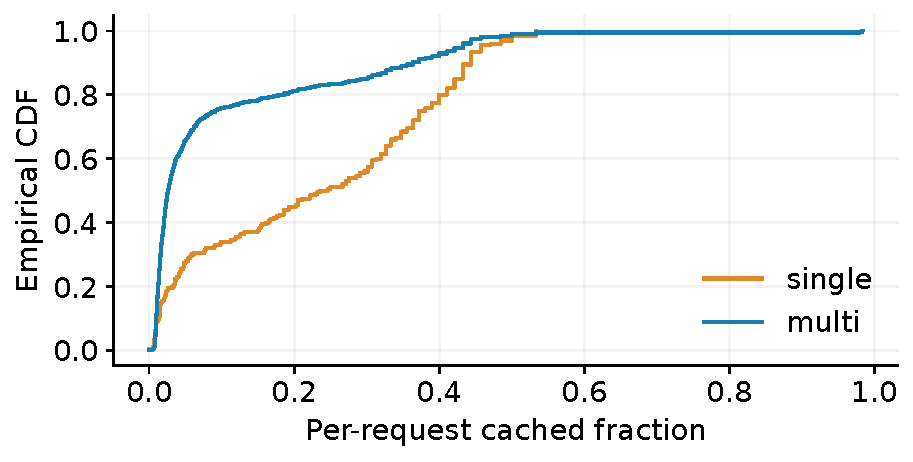
\includegraphics[width=.70\textwidth]{figures/m2_cdf_request.pdf}\hfill
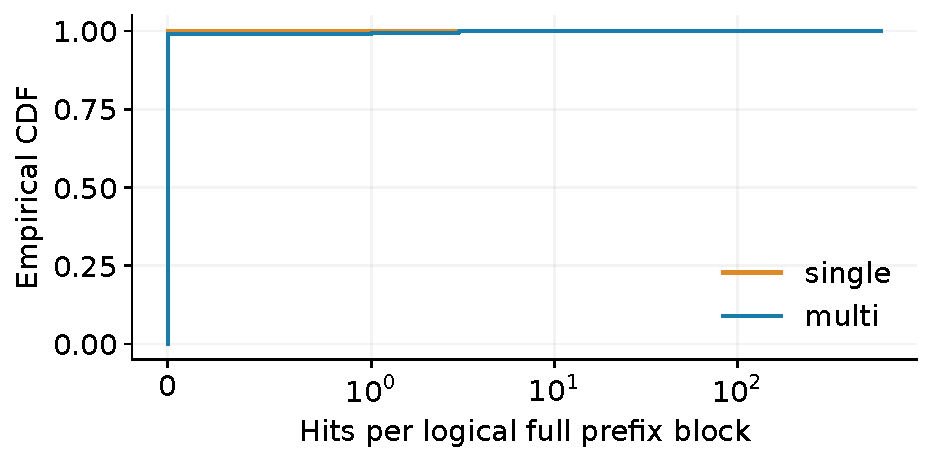
\includegraphics[width=.70\textwidth]{figures/m2_cdf_blocks.pdf}\hfill
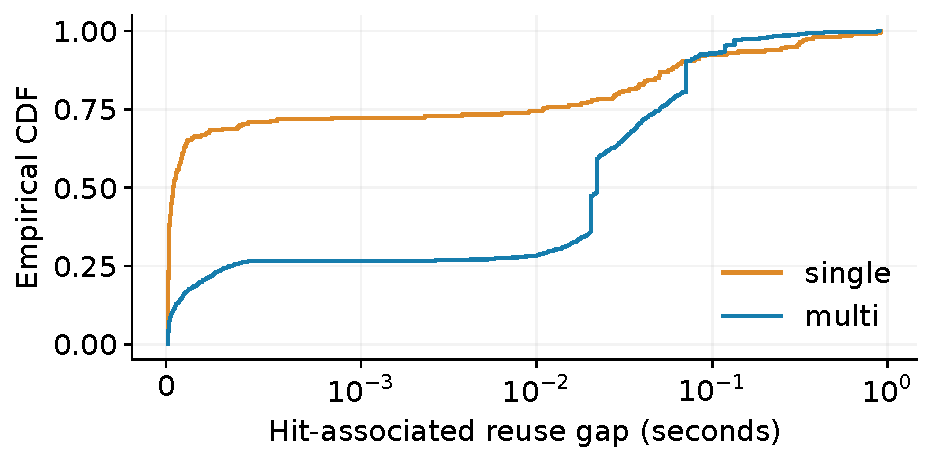
\includegraphics[width=.70\textwidth]{figures/m2_cdf_gaps.pdf}
\caption{M2 descriptive CDFs, LRU/block 16/0.05\,GiB/seed 0. Request fractions, logical-block hits including zero hits, and successful-hit-associated wall-clock gaps have different populations.}
\end{figure*}
\begin{figure*}[t]\centering
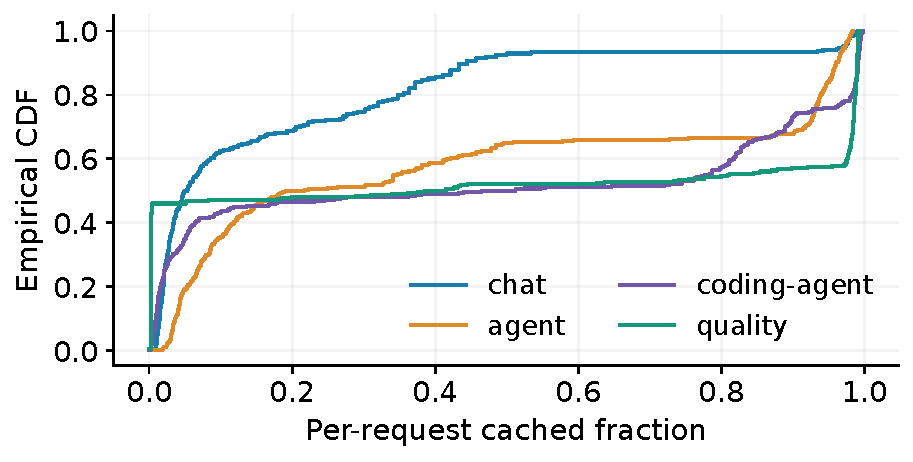
\includegraphics[width=.70\textwidth]{figures/m3_cdf_request.pdf}\hfill
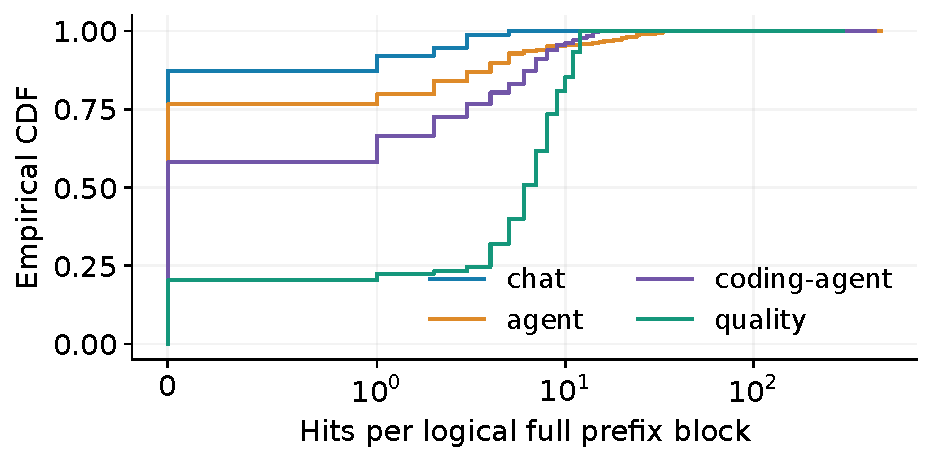
\includegraphics[width=.70\textwidth]{figures/m3_cdf_blocks.pdf}\hfill
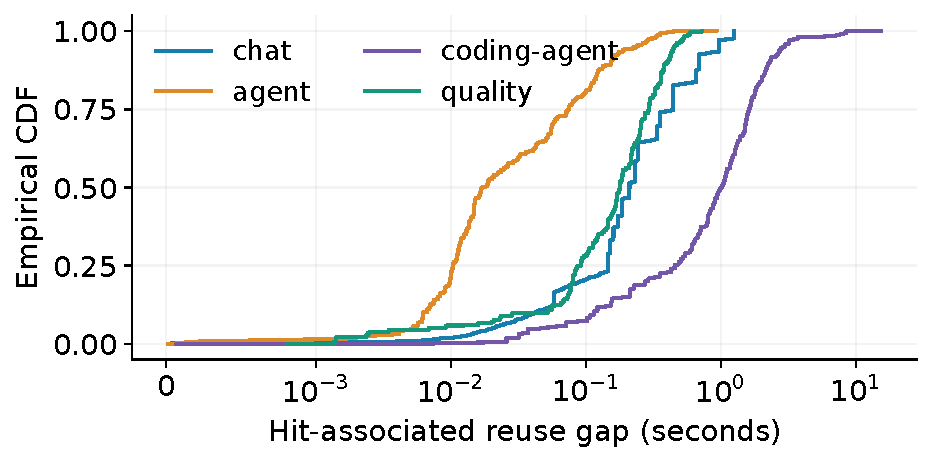
\includegraphics[width=.70\textwidth]{figures/m3_cdf_gaps.pdf}
\caption{Task 1 representative LRU seed 0 distributions; source-specific contexts/capacities differ. The separate planned-prompt diagnostic uses nominal arrival times and no cache model; it is distinct from these hit-conditioned wall-clock gaps.}
\end{figure*}
\begin{figure*}[t]\centering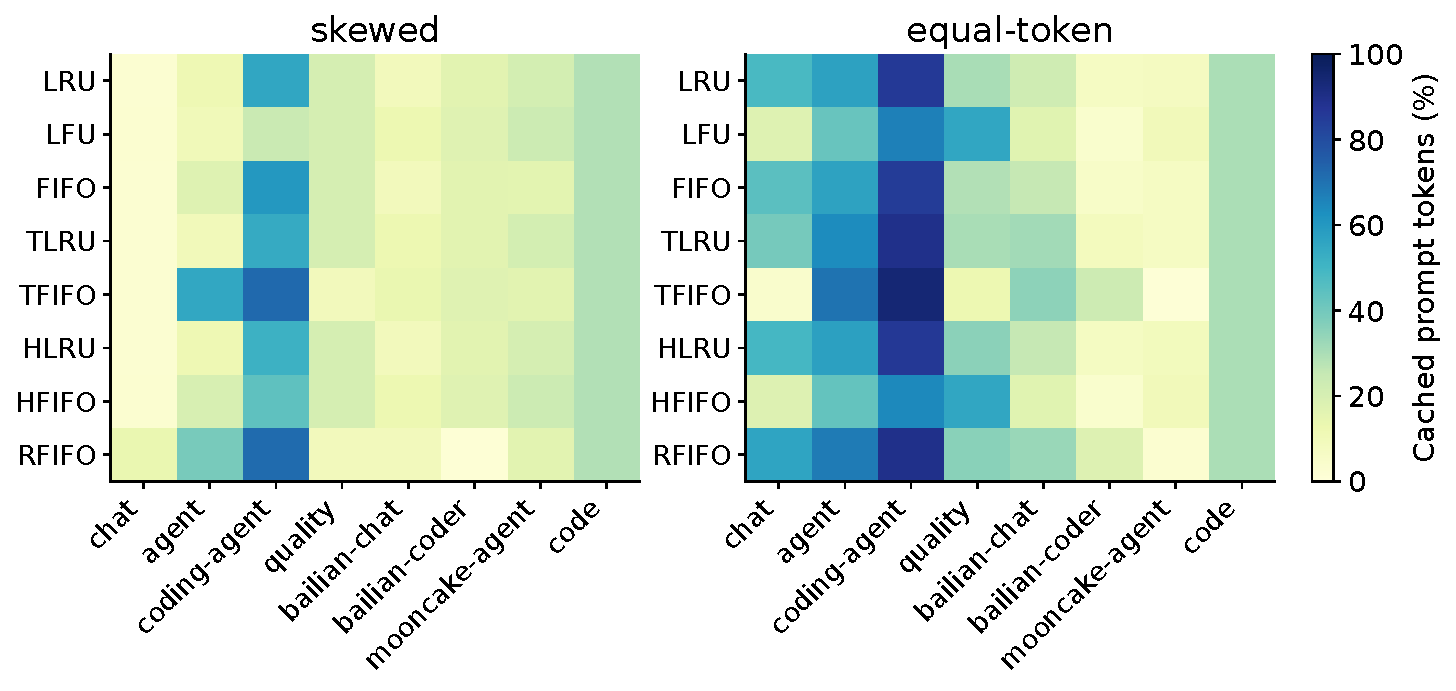
\includegraphics[width=.99\textwidth]{figures/mixed_by_workload.pdf}
\caption{New mixed per-label token-weighted sharing; improvements in an aggregate can conceal harm to individual categories.}
\end{figure*}
\begin{figure*}[t]\centering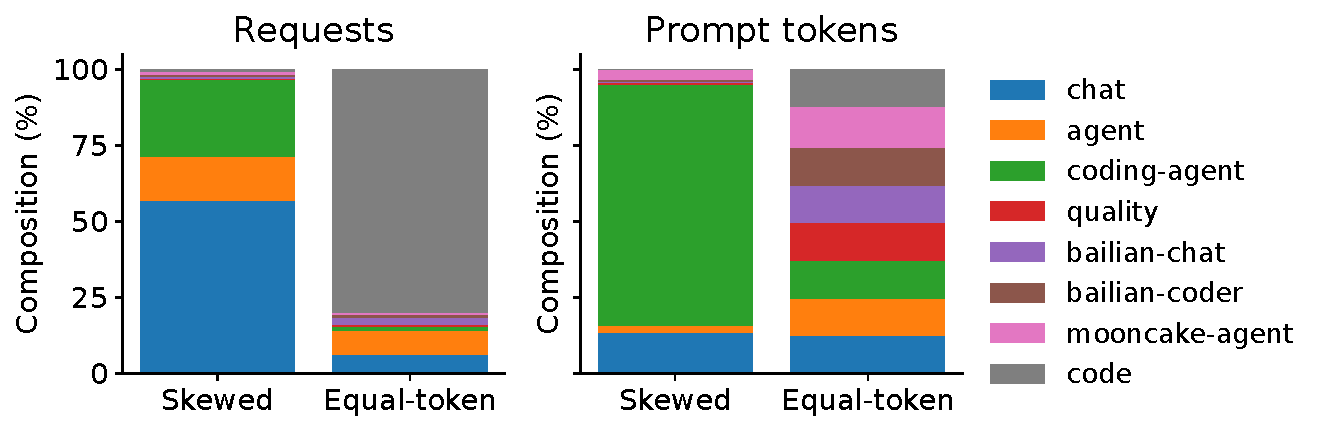
\includegraphics[width=.99\textwidth]{figures/mixed_composition.pdf}
\caption{Request and prompt-token composition are distinct. Equal-token cohorts preserve causal prefixes and overshoot by their last selected turn.}
\end{figure*}

\begin{figure*}[t]\centering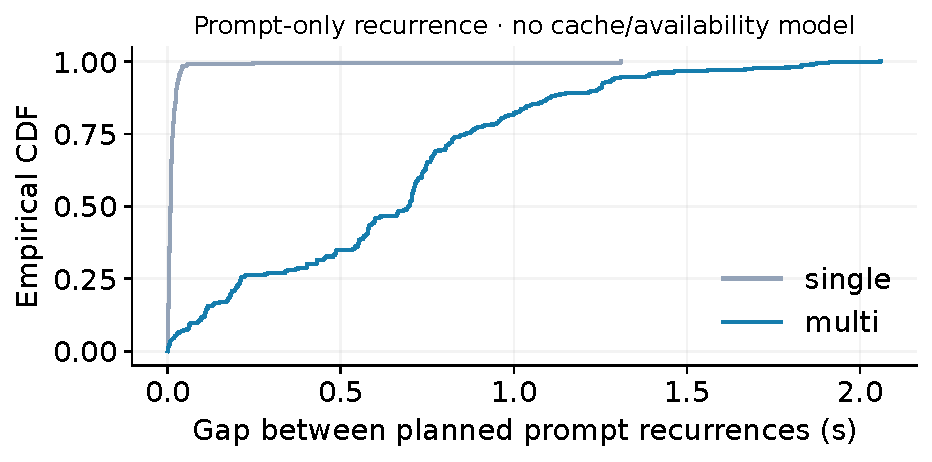
\includegraphics[width=.65\textwidth]{figures/m2_planned_prompt_recurrence.pdf}
\caption{Policy-independent nominal prompt recurrence, M2/block 16/seed 0. Population: repeated full prompt blocks; no decode-produced blocks, capacity, completion-time availability or actual dispatch model. This is neither a realized-hit CDF nor a full-serving upper bound.}
\end{figure*}
\section{Policy State and Pseudocode}
\begin{table*}[t]\centering\small
\caption{Source-grounded policy comparison. Only unused blocks are candidates; protection is a victim preference, not pinning.}
\begin{tabular}{lp{.34\textwidth}p{.38\textwidth}}\toprule
Policy & Candidate priority / order & State and admission / expiry\\\midrule
LRU & Oldest access; deeper prefix on a tie & Recency metadata\\
LFU & Lowest frequency, then recency/order & Access frequency survives pin/release\\
FIFO & Oldest original insertion serial & Access/pinning does not refresh serial\\
TLRU & Static low, protected, shared tiers; recency & Agent/Bailian labels; shared tier last; hold8\,s and budget 1\\
TFIFO & Same static tiers; FIFO & Same labels/shared tier; no hold/budget expiry\\
HLRU & Unhit/expired before fresh reused; recency & First own hit; hold8\,s and budget 1\\
HFIFO & Unhit before hit; FIFO & First own hit; no expiry\\
RFIFO & Low before admitted; FIFO & Full100 resolved outcomes/label, $\ge5\%$ hits admit future blocks; no retroactive low-tier promotion\\\bottomrule
\end{tabular}\end{table*}
TLRU: classify each unused cached block as fixed, protected or cross-label shared; demote the oldest protected candidate to fixed competition when expired or above budget; evict the earliest tier's LRU victim. TFIFO: use static label tiers and FIFO serials without time/budget demotion. HFIFO/HLRU: begin unhit; promote on first own reuse; clear hit state on physical reuse; use FIFO or time-limited recency order. RFIFO: resolve a residency once on first hit or unhit eviction; append outcomes to each associated label's last100 entries; admit future blocks when any full label window reaches5\% hits; evict low before admitted tier by insertion order. If no low blocks remain, protected blocks are still evictable. Active pinned blocks are outside the evictor.

Metadata includes label sets, insertion/frequency/hit state, versions and tier heaps; RFIFO additionally uses bounded per-label windows. Typical operations are logarithmic heap operations plus label/window work; lazy stale entries and periodic linear rebuilds mean worst-case latency is not strictly logarithmic. We do not report measured byte/CPU overhead or unavailable promotion counters. Mixed eviction counts come from a successful-allocation wrapper; older runs have no such counter. Full source mapping and limitations are in \texttt{POLICY\_DETAILS.md}.

\section{Team Contributions and Source History}
Author order is Thomas Lin, Yu-Ting Chung, Patrick Chiou and Yu-Xin Lai; all are Rice University affiliates. Complete project history is available and the assigned upstream baseline is an ancestor. Thomas Lin's visible commits cover mixed construction, label transport and custom policies. Yu-Ting Chung's cover original simulator integration/optimization and expanded heterogeneous adapters/traces. Yu-Xin Lai's cover client timing/templates/ID matching, single/multi replay, metrics, FIFO/LFU and M2 sweep automation. Patrick Chiou's cover initial Task 1 work and the AI-assisted final report/presentation, testing, bug fix and integration in this session. These are component-level evidence and assigned responsibilities, not effort percentages or presenter assignments. Human review details require confirmation; no corresponding author is designated.

\section{Significant AI Prompts}
The final user instructions asked to complete simulator validation, recover or execute missing M2 and mixed experiments, minimally repair unresolved multiprocessing label transport, preserve original artifacts/history, use the four confirmed authors/emails, produce a six-page MLSys-style main report and update the required15-minute presentation. The presentation supplement specified15 main slides,13min30\,s timing, approximately 1,450--1,600 spoken English words, instructor Q\&A and TA reproduction instructions. Earlier requests asked for initial Task 1 code/report, necessary-only Git changes, and a subsequent read-only evidence audit. These are summaries of actual available prompts, not reconstructed historical prompts from other team members. Selected verbatim instructions were: ``Implement the minimal correct fix. Do not simply discard the workload argument or globally disable multiprocessing to hide the problem.'' Another instruction was: ``Do not rerun valid experiments unnecessarily.'' The final request also stated: ``Do not fabricate results, contributions, citations, or validation evidence.'' Complete provided final-task and presentation prompts are archived verbatim in the accompanying \texttt{AI\_PROMPTS.md}; historical prompts from other contributors are not reconstructed.
\end{document}
